\chapter{Formulación del Problema de Optimización}

Con el fin de crear un contexto formal y bien definido para el problema de optimización del MLR diseñado, se tomó el enfoque propuesto en \cite{arora2012}. En este se identifican por separado dos métodos que pueden utilizarse para obtener un diseño que satisfaga ciertos criterios: un método convencional, y un método óptimo, como se muestra en la Fig. \ref{fig:conventionaloptimumdesign}.

\begin{figure}[t]
\centering
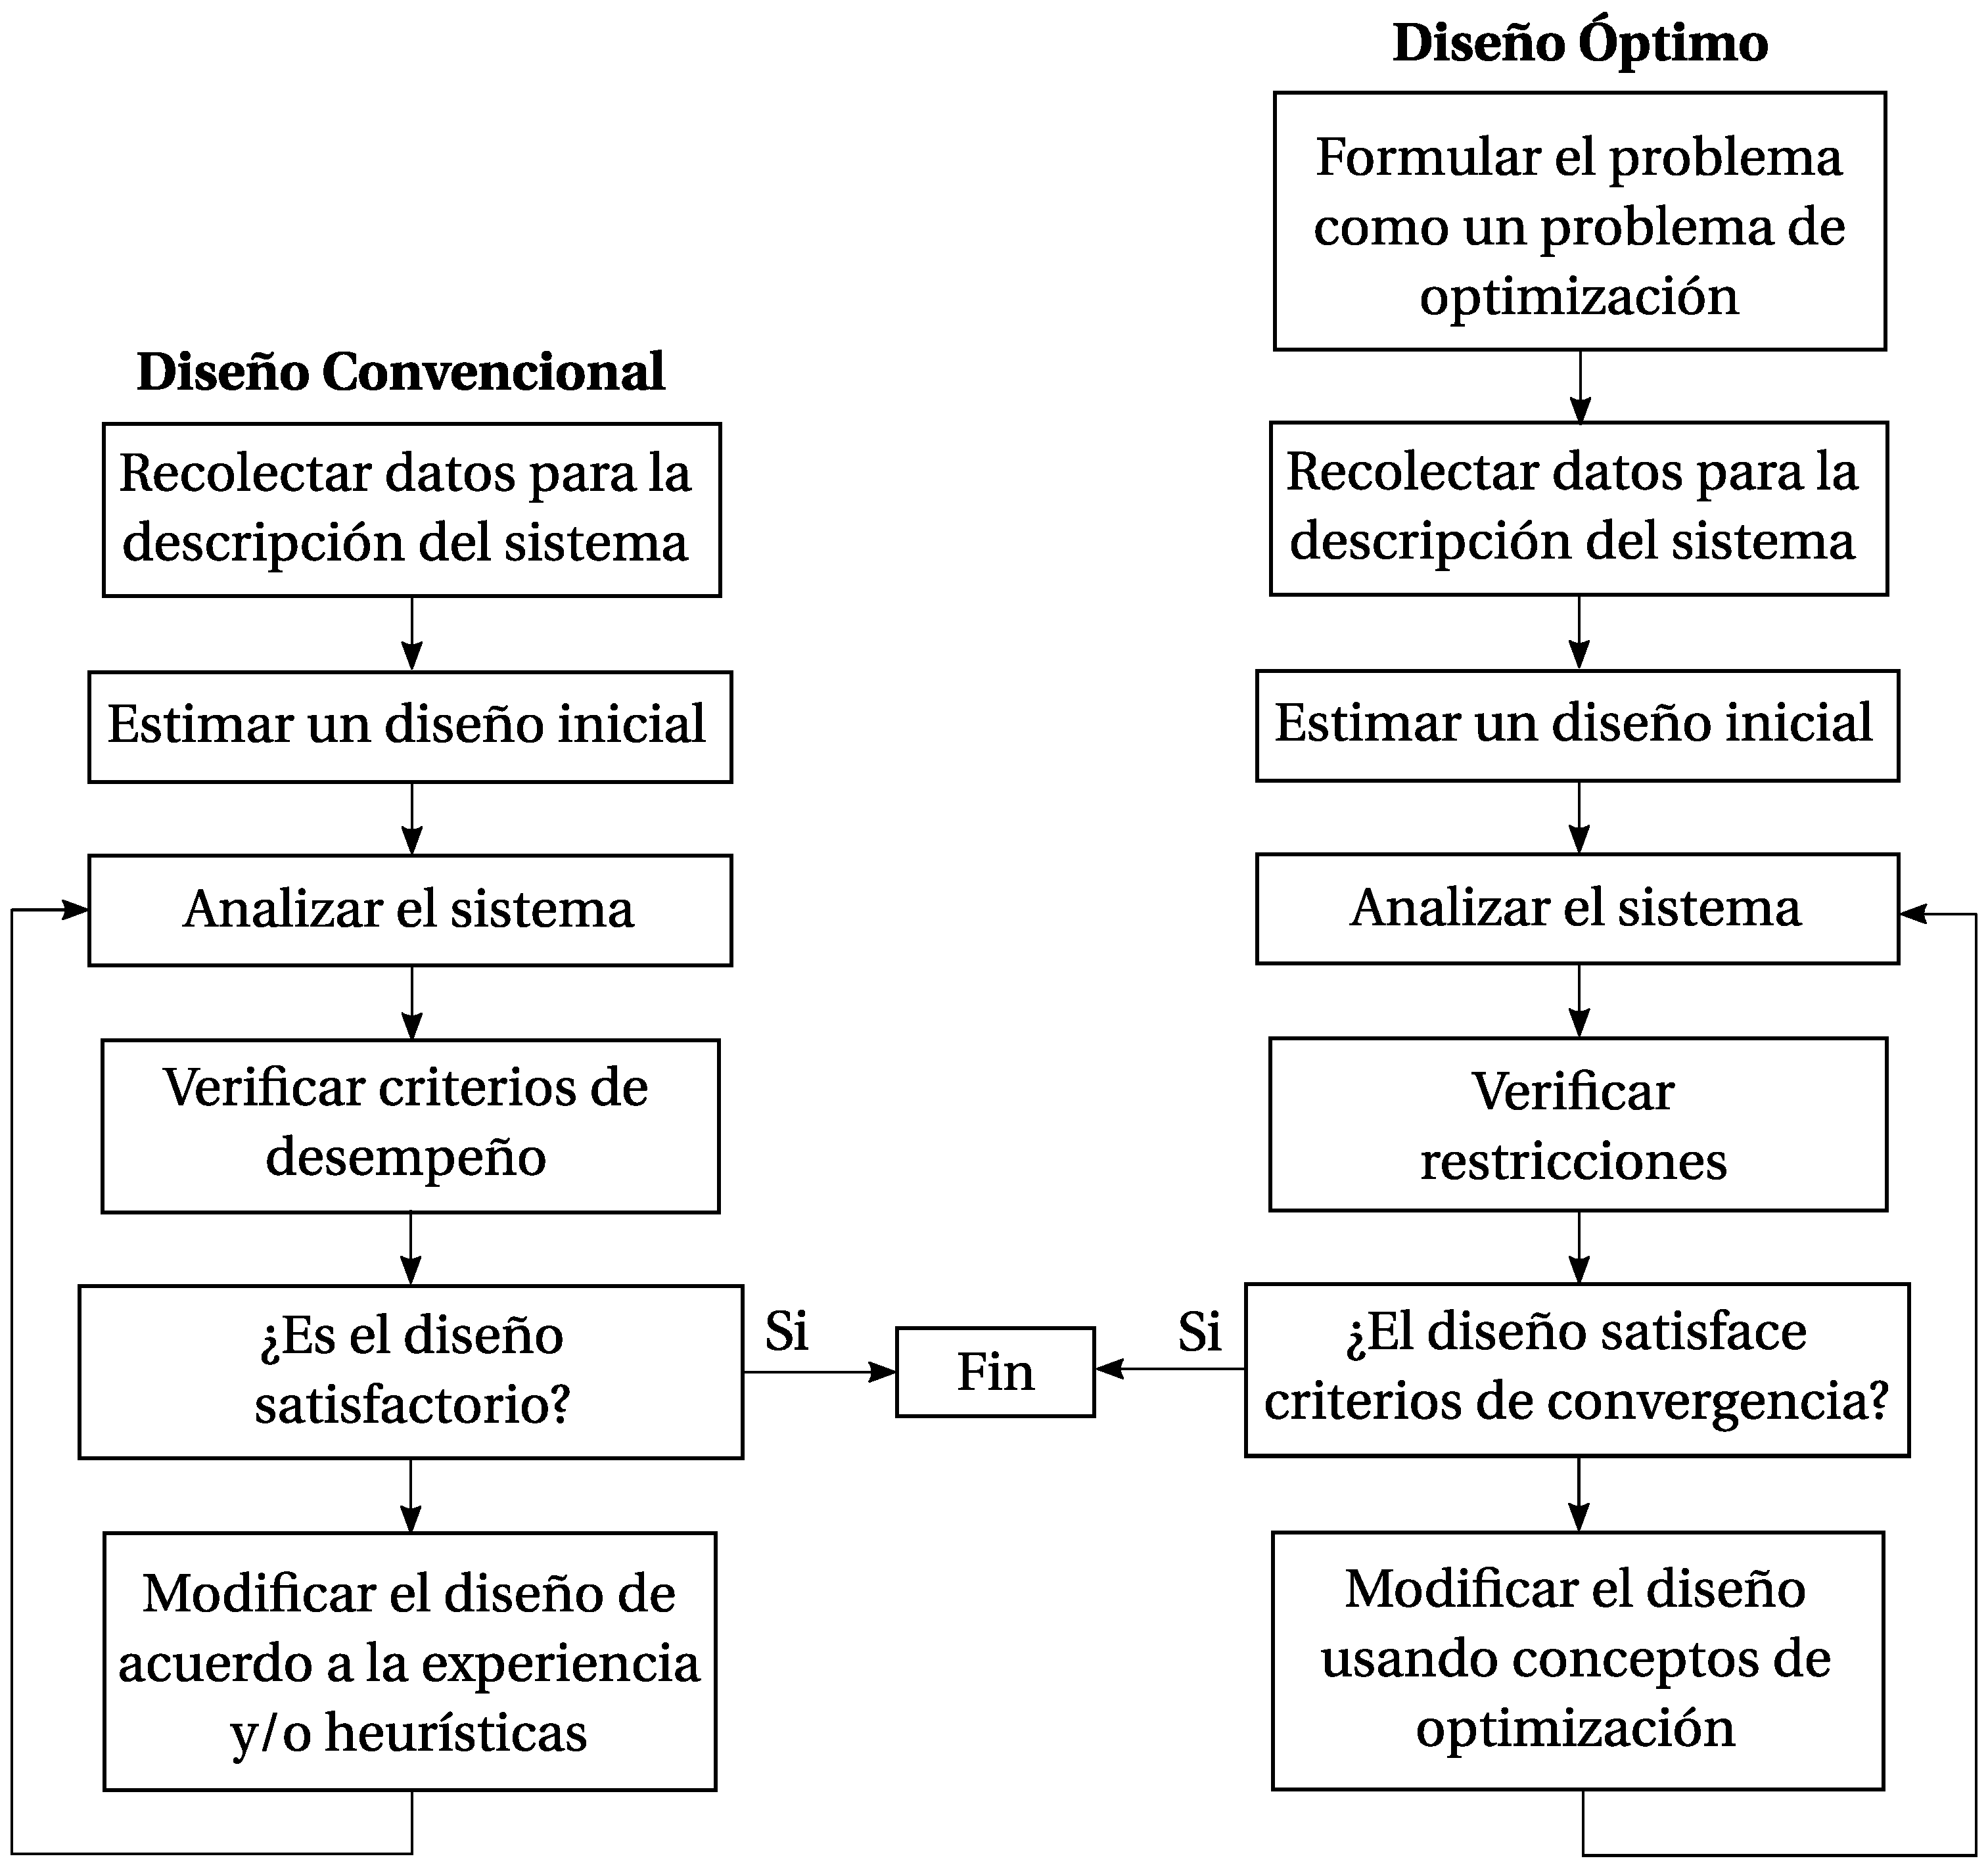
\includegraphics[scale=0.25]{../img/Formulacion_del_Problema_de_Optimizacion/conventionaloptimumdesign.eps}
\caption{Comparación entre el diseño convencional y óptimo. Adaptado de \cite{arora2012}.}
\label{fig:conventionaloptimumdesign}
\end{figure}

Es importante notar que ambos métodos son iterativos, pero el método de diseño óptimo es más formal tanto en la definición del problema como en la verificación de restricciones y la modificación del diseño, en la que se utilizan conceptos propios de la teoría de optimización, en contraste con la experiencia y las heurísticas utilizadas en el método convencional. Teniendo en cuenta lo anterior, puede observarse que el diseño inicial se obtuvo con base en un método de diseño convencional: la recolección de datos se realizó por medio de fórmulas, curvas y resultados de trabajos previos, a partir del cual se estimó un diseño inicial que posteriormente fue analizado por medio del FEM. El criterio de desempeño fue el requisito de potencia de 100 W, que al no ser cumplido inicialmente, hizo necesario modificar el diseño de acuerdo a lo observado en los resultados del FEM.

Una vez se obtuvo un diseño que cumpliera los requisitos de potencia, se procedió a aplicar los pasos de diseño óptimo como se muestran en la Fig. \ref{fig:conventionaloptimumdesign}. El primer paso consiste en la formulación del problema de optimización, que se ha descompuesto en diferentes partes que se desarrollan a continuación.

\section{Descripción del problema}
Se ha propuesto un diseño inicial para un MLR de 100 W, basado en un procedimiento en el cual se utilizaron expresiones analíticas aproximadas y resultados de trabajos relacionados, que fue mejorado a través de la experiencia y el análisis del motor a través del FEM, en lo que constituye un método de diseño convencional. Aunque este diseño inicial cumplió los requisitos de diseño, su eficiencia es demasiado baja.

Con base en este diseño inicial, se debe obtener un MLR que desarrolle una potencia mecánica de 100 W con una eficiencia mayor a la del diseño inicial. Se deberán definir restricciones sobre las dimensiones del motor con el fin de limitar su tamaño y peso.

\section{Recolección de datos e información}
A pesar de que se han propuesto expresiones analíticas para describir las propiedades electromagnéticas del MLR, el diseño convencional mostró que bajo condiciones de fuerte saturación es difícil predecir su validez. Por este caso, se utilizará un estudio estacionario en dos dimensiones utilizando el FEM, el cual es ampliamente utilizado en el estudio de las máquinas eléctricas debido a la fidelidad que brinda \cite{bianchi2011,boldea2015,gudelhofer2012,agarlita2013}.

\section{Selección de las variables de diseño}

En esta etapa se seleccionaron las variables que se consideraron relevantes para la descripción del sistema a diseñar. En general, al considerarse $n$ variables de diseño, cualquier posible selección de valores forma un vector de diseño
\begin{equation*}
\mathbf{x}=
(x_1, x_2, x_3, \ldots, x_n)
\end{equation*}
De esta forma, cualquier vector de diseño es un punto en el espacio de diseño $D$, tal que $\mathbf{x}\in D$ y $D \subset \mathbf{R}^n$.

Para el MLR, se encontró que pueden seleccionarse variables relacionadas con su geometría, así como variables eléctricas, tal como se encontró en trabajos relacionados \cite{mendrela2008,chayopitak2005,mohammadi2015,orlova2015}, en los cuales la selección de variables varía desde la geometría del primario, hasta la del secundario, con diferentes formas en ambos elementos. Durante el proceso de diseño se observó que la distancia del entrehierro, el paso polar y el ancho del motor tenían un efecto directo en la razón $L_d/L_q$. Se decidió dejar fija la distancia del entrehierro debido a que valores menores serían más complicados de fabricar, y valores mayores sólo disminuirían la razón mencionada. De esta forma, se definieron las dos primeras variables de diseño:
\begin{itemize}
\item $x_1$: Paso polar
\item $x_2$: Ancho del motor
\end{itemize}

Al obtener los resultados de eficiencia, se determinó que una de las razones para los bajos valores obtenidos fue la baja sección transversal de los conductores, que aumentaba su resistencia y por lo tanto las pérdidas en el cobre. Por lo tanto, se decidió que el área de las ranuras en el primario, la cual determina el área transversal de los conductores, debía ser incluida dentro de las variables del diseño. Debido a que existen varios parámetros en la geometría del primario que definen esta área, se definió la \textbf{razón ancho de ranura - paso de ranura}.

El ancho de ranura define la distancia horizontal de cada ranura en la que se posiciona el devanado en el primario, mientras que el paso de ranura es la distancia entre cada ranura del primario, que depende del paso polar. De esta forma, si la razón ancho de ranura - paso de ranura se define como
\begin{equation*}
\beta_s = \frac{b_s}{\tau_s}
\end{equation*}
entonces si $\beta_s\rightarrow 0$ el ancho de la ranura tenderá a 0, y si $\beta_s\rightarrow 1$, el ancho de la ranura tenderá a $\tau_s$, el cual es el máximo valor posible, como se muestra en la Fig. \ref{fig:bs2taus}.

\begin{figure}[t]
\centering
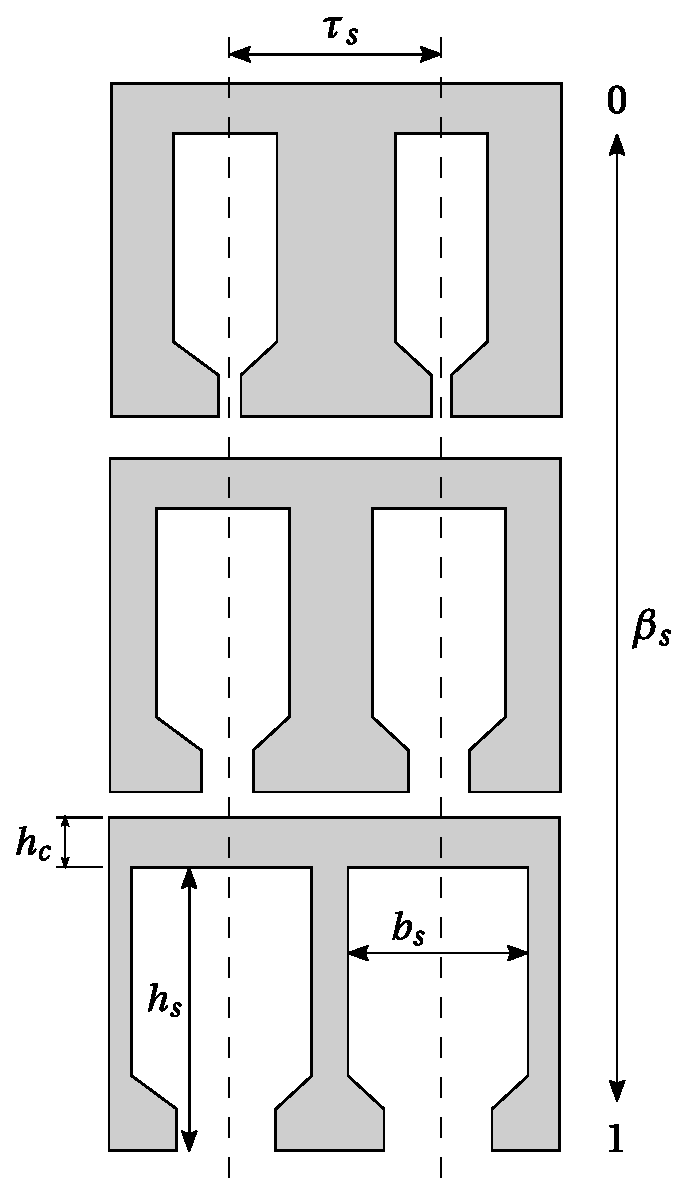
\includegraphics[scale=0.6]{../img/Formulacion_del_Problema_de_Optimizacion/bs2taus.eps}
\caption{Relación entre $\beta_s$ y la geometría del primario.}
\label{fig:bs2taus}
\end{figure}

Con respecto a esta variable, hay que tener en cuenta que valores demasiado bajos de $\beta_s$ producen conductores de menor diámetro, o incluso conductores con secciones de área transversal que no existen comercialmente. Por otro lado, valores demasiado altos de $\beta_s$ producen secciones más delgadas de material ferromagnético que son fácilmente susceptibles a la saturación.

Teniendo en cuenta lo anterior, se define la siguiente variable de diseño:
\begin{itemize}
\item $x_3$: Razón ancho de ranura - paso de ranura
\end{itemize}

Además del ancho de las ranuras, dos variables que tienen un efecto directo en la geometría son la altura posterior del núcleo $h_c$ y el alto de ranura $h_s$ (véase la Fig. \ref{fig:bs2taus}). Mientras que el alto de ranura influye de forma similar que el ancho en el área transversal resultante de los conductores, $h_c$ determina la cantidad de material ferromagnético utilizada en el circuito magnético del primario, lo cual puede mejorar el desempeño del motor frente a la saturación. Por lo tanto, se definieron las variables:
\begin{itemize}
\item $x_4$: Alto de ranura
\item $x_5$: Altura posterior del núcleo
\end{itemize}

La variación del paso polar afecta directamente la geometría del secundario laminado, aunque es posible modificar la forma de las láminas, como se sugiere en \cite{hamler1998}. Con el fin de no incrementar la dimensión del problema en una primera aproximación al mismo, se decidió trabajar con el mismo número de laminaciones (4) y ancho de las laminaciones (3.75 mm), mientras que el resto de las dimensiones de las láminas se varió de manera proporcional al paso polar.

Debido a que la definición de las anteriores variables afecta las inductancias de los ejes directo y en cuadratura, la ecuación fundamental del MLR sugiere que para valores constantes de corriente, el empuje desarrollado variará:
\begin{equation*}
F_x = \frac{3\pi}{2\tau}(L_d - L_q)I_d I_q
\label{devthrust}
\end{equation*}
Si se obtiene una diferencia entre $L_d$ y $L_q$ alta con los mismos valores de corriente, el empuje desarrollado será mayor, y consecuentemente la eficiencia del motor. Sin embargo, es posible que existan valores de las variables de diseño que producen un motor eficiente, pero que no cumple las especificaciones mínimas de potencia. Por esto, se decidió añadir la corriente de fase del motor como una variable de diseño adicional:
\begin{itemize}
\item $x_6$: Corriente de fase
\end{itemize}

Como se evidenció en el capítulo anterior, el flujo de enlace en el MLR es directamente proporcional al número de vueltas. Además, como se muestra en el apéndice B, el empuje desarrollado es directamente proporcional al cuadrado del flujo de enlace, por lo que para valores fijos de corriente, un mayor flujo de enlace se traduciría en mayor empuje con menores pérdidas en el cobre y por lo tanto, una mayor eficiencia. Sin embargo, un mayor número de vueltas se traduce en más material resistivo que eventualmente podría reducir la eficiencia al aumentar las pérdidas en el cobre. Este doble efecto sugirió la adición de la última variable de diseño:
\begin{itemize}
\item $x_7$: Número de vueltas por bobina
\end{itemize}

\section{Criterio de optimización}
Aunque es posible plantear un problema de optimización de múltiples objetivos orientado a encontrar un diseño óptimo con más de un criterio, como el peso, el torque y la eficiencia \cite{duan2013}; la eficiencia y la masa \cite{dubas2008}; o el empuje, la masa y el rizado en el empuje \cite{vaezzadeh2006}, de acuerdo a lo especificado en la descripción del problema, se quiere incrementar únicamente la eficiencia del motor. La ecuación \ref{devthrust} sugiere aumentar la diferencia entre las inductancias $L_d$ y $L_q$, lo cual produciría un motor más eficiente para los mismos valores de corriente, y aún más si la corriente de fase pudiera reducirse. Sin embargo, en lugar de esta diferencia, históricamente se ha preferido la razón $L_d/L_q$ debido a consiste en un indicador más apropiado con respecto al desempeño de un MLR, en términos del factor de potencia, el rango de velocidad alcanzado con valores de potencia constantes y la respuesta dinámica del motor \cite{staton1993}, la cual es una idea que se aplica hasta años recientes \cite{boldea2013}.

Por otro lado, otros trabajos sugieren definir un criterio de optimización en el cual se tiene una única función objetivo pero que reúne de forma directa diferentes características de interés, asignando potencias de acuerdo a la prioridad que se le desea dar a determinada cantidad \cite{dong2014,shiri2012}.

Con el fin de incluir los aspectos de interés en el criterio de optimización, se decidió definir un criterio de optimización que tuviera en cuenta de forma directa el empuje desarrollado y las pérdidas en el cobre, asignando una mayor prioridad al empuje. De esta forma, la función objetivo a maximizar se definió como
\begin{equation*}
f(\mathbf{x}) = \frac{F_x^2}{P_j}
\end{equation*}
donde $F_x$ es el empuje desarrollado en newton y $P_j$ son las pérdidas en el cobre, en vatios.

\section{Formulación de restricciones}

Las restricciones del problema permiten establecer valores mínimos y máximos para las variables o las funciones del sistema, con el fin de restringir el conjunto de posibles soluciones a un grupo de soluciones viables desde un punto de vista técnico. Esto indica que los valores relacionados con la geometría y los materiales del conunto de soluciones evaluadas cumplirán garantizarán que no se tienen soluciones inviables como conductores extrmadamente delgados, corrientes muy elevadas o uso de grandes cantidades de material en el núcleo. A partir de estas restricciones, se calcularon límites inferiores y superiores para cada una de las variables de diseño, como se muestra en la Tabla \ref{table:restrictions}.

\begin{table}[!hb]
\centering
\caption{Restricciones del problema de optimización.}
\label{table:restrictions}
\begin{tabular}{c c c}
\hline\hline\\
Variable & Restricción\\
\hline\\
Paso polar & 5 cm $\leq x_1 \leq$ 12 cm\\
Ancho del motor & 5 cm $\leq x_2 \leq$ 14 cm\\
Razón ancho de ranura - paso de ranura & 0.4 $\leq x_3 \leq$ 0.7\\
Alto de ranura & 2 cm $\leq x_4 \leq$ 4 cm\\
Altura posterior del núcleo & 5 mm $\leq x_5 \leq$ 20 mm\\
Corriente de fase & 1 A $\leq x_6 \leq$ 5 A\\
Vueltas por fase & 25 $\leq x_7 \leq$ 100\\
\hline\hline\\
\end{tabular}
\end{table}

\section{Formulación del problema}
De acuerdo a lo estipulado en la descripción del problema y la sección acerca de la recolección de datos e información, se busca encontrar valores para las variables de diseño:
\begin{itemize}
\item $x_1$: Paso polar
\item $x_2$: Ancho del motor
\item $x_3$: Razón ancho de ranura - paso de ranura
\item $x_4$: Alto de ranura
\item $x_5$: Altura posterior del núcleo
\item $x_6$: Corriente de fase
\item $x_7$: Número de vueltas por bobina
\end{itemize}
con el fin de maximizar la función objetivo
\begin{equation*}
f(\mathbf{x}) = \frac{F_x^2}{P_j}
\end{equation*}
sujeto a las restricciones listadas en la Tabla \ref{table:restrictions}.

\section{Conclusiones}
La formulación del problema como fue expuesta anteriormente buscó establecer un contexto claro y definido para la definición del problema de optimización de forma que pudiera ser visto como un caso genérico al que pueden aplicarse diferentes métodos de optimización. Es necesario, sin embargo, hacer una nota final relacionada con la recolección de datos e información del problema en específico.
Cualquier posible evaluación de un vector de diseño arbitrario $\mathbf{x}_k$ requiere de la aplicación del FEM para la obtención del valor de la función objetivo en el punto, $f(\mathbf{x}_k)$. Esto quiere decir que no se cuenta con una expresión analítica para la función objetivo en términos de las variables de diseño, por lo que cualquier método de optimización que la requiera queda, en primera instancia, descartado.

Podría pensarse, por lo tanto, que aquellos métodos que no hacen uso de una función explicita de las variables de diseño, pueden ser aplicables directamente para la solución de este problema. Sin embargo, desde el punto de vista práctico, esta no puede ser una alternativa viable. Suponiendo inicialmente que se tiene un espacio de diseño de una dimensión, y quieren tomarse $k$ muestras de la función objetivo a lo largo de esta única dimensión, entonces es necesario hacer $k$ evaluaciones de la función objetivo. Por lo tanto, por cada dimensión que se añada al problema, el número de evaluaciones se multiplica por $k$, si se quiere cubrir el espacio de diseño de la misma forma uniforme. Esto quiere decir que para un número $n$ de variables, el número de evaluaciones requerido es $k^n$. Para la situación del MLR tratada en específico, $n$ = 7, que con tan solo $k$ = 3 requiere de 2187 evaluaciones de la función objetivo. Este problema, llamado por Bellman como \textit{la maldición de la dimensionalidad} \cite{bellman1957}, limita la aplicabilidad directa de métodos computacionalmente costosos que evalúan la función objetivo a través de herramientas como el FEM, donde una sola evaluación puede tomar desde minutos a varias horas.

Estas consideraciones hicieron necesaria la aplicación de una herramienta que surge como alternativa en tales casos: el \textbf{metamodelado}. Su descripción, aplicación y resultados se muestran en el siguiente capítulo.

\bibliographystyle{ieeetr}
\bibliography{../refs}